\documentclass[10pt,a4paper]{article}

\usepackage[margin=2.3cm]{geometry}
\usepackage{amsmath,amssymb,amsthm}
\usepackage{booktabs}
\usepackage{array}
\usepackage[hidelinks]{hyperref}
\usepackage{microtype}
\usepackage{xcolor}
\usepackage{listings}

\lstset{
  language=Python,
  basicstyle=\small\ttfamily,
  commentstyle=\color{gray}\itshape,
  keywordstyle=\bfseries,
  showstringspaces=false,
  columns=fullflexible,
  keepspaces=true,
  xleftmargin=1.6em,
  aboveskip=\medskipamount,
  belowskip=\medskipamount,
}

% --- figures: TikZ/pgfplots; data tables precomputed by nop_figs/make_data.py ---
\usepackage{tikz}
\usepackage{pgfplots}
\pgfplotsset{compat=1.17}
\usepgfplotslibrary{colormaps}
\usetikzlibrary{arrows.meta, positioning}
\definecolor{cdata}{RGB}{36,90,160}   % blue
\definecolor{cnoise}{RGB}{192,80,60}  % red
\definecolor{cflow}{RGB}{0,135,125}   % teal
\pgfplotsset{
  dfm/.style={
    label style={font=\footnotesize},
    tick label style={font=\scriptsize},
    title style={font=\footnotesize},
    legend style={font=\scriptsize, draw=gray!40},
    axis line style={gray!70},
    tick style={gray!70},
  },
}

\newtheorem{lemma}{Lemma}
\newtheorem{proposition}{Proposition}
\newtheorem{exercise}{Exercise}

\newenvironment{recap}
{\par\medskip\noindent\begin{quote}\small\textbf{The story so far.}\itshape\;}
{\end{quote}\medskip}

\newcommand{\R}{\mathbb{R}}
\newcommand{\N}{\mathbb{N}}
\newcommand{\E}{\mathbb{E}}
\newcommand{\dd}{\mathrm{d}}
\newcommand{\G}{\mathcal{G}}
\newcommand{\A}{\mathcal{A}}
\newcommand{\U}{\mathcal{U}}
\newcommand{\V}{\mathcal{V}}
\newcommand{\K}{\mathcal{K}}
\newcommand{\F}{\mathcal{F}}
\newcommand{\id}{\mathrm{id}}
\newcommand{\mesh}{\mathcal{M}}

\title{Functions In, Functions Out:\\
\large Neural Operators, Slowly}
\author{Matthew Willetts\\{\small with assistance from Codex and Claude}}
\date{v0.1 --- June 2026}

\begin{document}
\maketitle

\begin{abstract}
\noindent Neural networks learn maps between vectors. Scientific computing is
full of maps between \emph{functions}: a permeability field goes in and a
pressure field comes out; an initial condition goes in and a future state
comes out; a boundary shape goes in and a stress field comes out. These notes
develop neural operators from that mismatch. The unifying move is to
replace dense matrices by \emph{operators} --- usually integral operators ---
and share their parameters across discretizations. DeepONets, Fourier neural
operators, graph neural operators, low-rank operators, and physics-informed
neural operators then become different answers to the same questions: how is
the input function observed, how is nonlocal information mixed, which basis or
mesh carries the kernel, and where is the physics loss imposed? The governing
principle is not that neural operators magically solve PDEs. It is that a
trained model amortizes an entire \emph{solution operator}: expensive data
generation happens once, then a new PDE instance is evaluated by a forward
pass.
\end{abstract}

\tableofcontents

\section{The problem: a solver is an operator}

Start with the object numerical analysts already own. Consider a parametric
PDE on a domain $D \subset \R^d$,
\begin{equation}
  \mathcal{L}_a u = f, \qquad \mathcal{B}u = g,
\label{eq:pde}
\end{equation}
where the coefficient, forcing, initial condition, or boundary data is called
$a$. For each admissible $a$ there is a solution $u$. Abstract away the
algorithm used to find it and what remains is the \textbf{solution operator}
\begin{equation}
  \G^\dagger : \A \to \U, \qquad a \mapsto u.
\label{eq:solution-operator}
\end{equation}
Here $\A$ and $\U$ are function spaces: perhaps
$a \in L^\infty(D)$ and $u \in H^1(D)$ for elliptic problems, or
$a = u_0$ and $\G^\dagger(a) = u(\cdot,T)$ for an evolution equation.

A classical solver approximates \eqref{eq:solution-operator} one input at a
time. Give it a new coefficient field, run Newton, multigrid, finite elements,
or a spectral code again. A neural operator tries to learn the whole map
\eqref{eq:solution-operator} from examples
\[
  \{(a_j, u_j)\}_{j=1}^N,
  \qquad u_j = \G^\dagger(a_j),
\]
so that a new input function is handled by one forward pass. The bargain is
clear:
\begin{center}
\emph{Pay for many high-quality solves during training; amortize them over
many future queries.}
\end{center}
If you only need one solve, use the solver. If you need millions of solves
inside design, control, data assimilation, uncertainty quantification, or a
larger simulator, the operator viewpoint becomes natural.

\subsection{Why ordinary networks are the wrong default}

One brute-force plan is to discretize $a$ and $u$ on a fixed grid and train a
standard network
\[
  \R^{m} \to \R^{m}, \qquad (a(x_1),\ldots,a(x_m)) \mapsto
  (u(x_1),\ldots,u(x_m)).
\]
This works as a regression problem, but it has the wrong type signature. The
input and output dimensions are artifacts of the mesh. Change the resolution,
move the points, or evaluate on an irregular grid and the architecture no
longer even has the right shape. Worse, the network can learn grid-specific
aliases: a map from arrays to arrays rather than a map from functions to
functions.

The objection covers CNNs too, more subtly than it covers MLPs. A
convolutional kernel is defined in \emph{pixels}: refine the mesh by a
factor of two and the same $3 \times 3$ stencil now sees half the physical
distance --- same parameters, different operator. A CNN is
resolution-\emph{shaped}, not resolution-\emph{aware}. (Contrast the
Fourier parameterization of Section~\ref{sec:fno}, whose learned weights
attach to physical frequencies: refining the grid adds representable modes
without touching the ones already learned.)

Neural operators keep the mesh as a \emph{way of observing} a function, not as
the mathematical object being learned. The same parameters should make sense
on a coarse grid, a fine grid, and often on different point clouds. This is
the slogan called \textbf{discretization invariance}. It does not mean
``accuracy is independent of resolution.'' It means the learned rule is
defined before a particular discretization is chosen.

\begin{recap}
The target is not a single PDE solution but the solution operator
$\G^\dagger : a \mapsto u$. Ordinary networks learn maps between arrays and
therefore inherit the training grid as part of their type. Neural operators
try to learn a mesh-independent rule whose inputs and outputs are functions,
with arrays serving only as samples of those functions.
\end{recap}

\section{The schema}
\label{sec:schema}

A neural operator has the same skeleton as a feed-forward network:
\[
  \text{lift} \quad \longrightarrow \quad
  \text{mix + nonlinearity repeatedly} \quad \longrightarrow \quad
  \text{project}.
\]
The difference is that the hidden states are functions
(Figure~\ref{fig:schema}).

\paragraph{Lift.}
Pointwise embed the input function and coordinates into a channel-valued
function:
\begin{equation}
  v_0(x) = P\big(a(x), x\big) \in \R^c.
\label{eq:lift}
\end{equation}
The coordinate $x$ is usually included because a translation-invariant kernel
alone cannot know where the boundary is, where coefficients change, or which
part of the domain it is seeing.

\paragraph{Operator layer.}
Alternate local channel mixing, nonlocal integral mixing, and a pointwise
nonlinearity:
\begin{equation}
  v_{\ell+1}(x)
  = \sigma\!\left(
      W_\ell v_\ell(x)
      + \int_D \kappa_\ell(x,y)\,v_\ell(y)\,\dd y
      + b_\ell(x)
    \right).
\label{eq:no-layer}
\end{equation}
This is the core neural-operator layer. $W_\ell$ is an ordinary matrix on
channels. The integral term is the operator analogue of a dense layer or a
convolution: it moves information from every $y$ to every $x$.

\paragraph{Project.}
Return to the desired output channels:
\begin{equation}
  \G_\theta(a)(x) = Q(v_L(x)).
\label{eq:project}
\end{equation}

\begin{figure}[t]
\centering
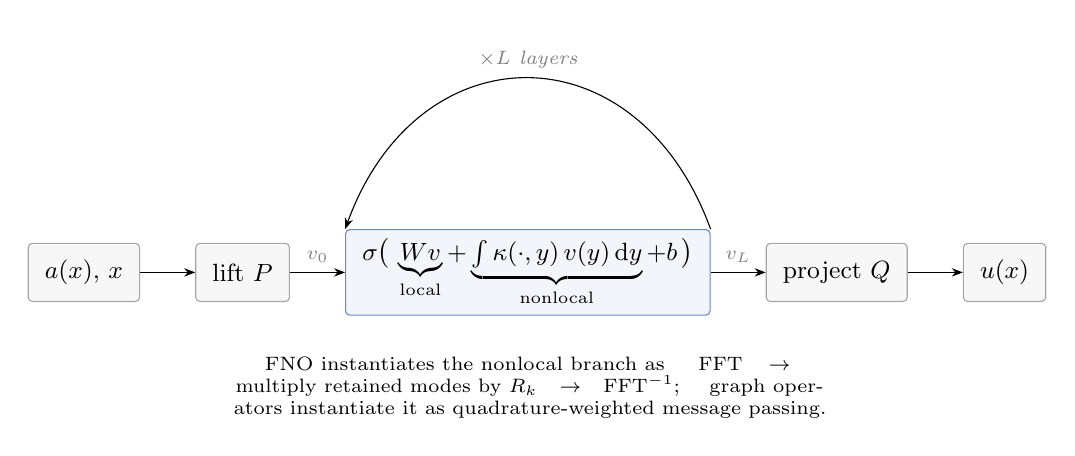
\begin{tikzpicture}[
  font=\small,
  box/.style={draw=gray!70, rounded corners=1.5pt, minimum height=2.1em,
    inner xsep=6pt, fill=gray!6},
  opbox/.style={draw=cdata!70, rounded corners=1.5pt, minimum height=2.1em,
    inner xsep=6pt, fill=cdata!6},
  lab/.style={font=\scriptsize\itshape, gray},
  >={Stealth[length=4pt]},
  node distance=5mm and 7mm,
]
\node[box] (a) {$a(x),\,x$};
\node[box, right=of a] (lift) {lift $P$};
\node[opbox, right=of lift] (layer)
  {$\sigma\big(\,\underbrace{W v}_{\text{local}}
   + \underbrace{\textstyle\int \kappa(\cdot,y)\,v(y)\,\dd y}_{\text{nonlocal}}
   + b\,\big)$};
\node[box, right=of layer] (proj) {project $Q$};
\node[box, right=of proj] (u) {$u(x)$};
\draw[->] (a) -- (lift);
\draw[->] (lift) -- node[above, lab] {$v_0$} (layer);
\draw[->] (layer) -- node[above, lab] {$v_L$} (proj);
\draw[->] (proj) -- (u);
\draw[->] (layer.north east) to[out=110, in=70, looseness=1.5]
  node[above, lab] {$\times L$ layers} (layer.north west);
\node[below=4mm of layer, font=\scriptsize, text width=10.2cm, align=center]
  {FNO instantiates the nonlocal branch as
   $\;\mathrm{FFT} \to \text{multiply retained modes by } R_k \to
   \mathrm{FFT}^{-1}$; \quad
   graph operators instantiate it as quadrature-weighted message passing.};
\end{tikzpicture}
\caption{The neural-operator schema. All hidden states are
\emph{functions}; the only structural difference from a feed-forward
network is that the dense matrix inside each layer has become an integral
kernel. The named architectures of the table below differ in how that
kernel is parameterized and evaluated.}
\label{fig:schema}
\end{figure}

\paragraph{Discretize only at execution time.}
On points $x_1,\ldots,x_m$, the integral in \eqref{eq:no-layer} becomes a
quadrature rule,
\begin{equation}
  \int_D \kappa(x_i,y)v(y)\,\dd y
  \;\approx\;
  \sum_{j=1}^m \kappa(x_i,x_j)v(x_j)w_j.
\label{eq:quadrature}
\end{equation}
The weights $w_j$ belong to the discretization, not to the learned operator.
This is the smallest mathematical difference between a neural operator and a
network that merely happens to process a grid.

\paragraph{Sanity check: fixed mesh.}
If the mesh is fixed forever, \eqref{eq:quadrature} is just a matrix
multiplication:
\[
  v_i' = \sum_j A_{ij} v_j,
  \qquad
  A_{ij} = \kappa(x_i,x_j)w_j.
\]
Nothing mystical has happened. The claim is not that a neural operator
escapes finite-dimensional computation; it plainly does not. The claim is
that the entries of the matrix are \emph{samples of a rule} defined before
the mesh was chosen. Refine the grid and you do not invent a new layer of a
new size; you resample the same kernel and change the quadrature weights.
That is the difference between learning an array-to-array map and
learning an operator.

\subsection{The architectures in one table}

\begin{center}
\footnotesize
\begin{tabular}{@{}>{\raggedright\arraybackslash}p{2.4cm}>{\raggedright\arraybackslash}p{4.2cm}>{\raggedright\arraybackslash}p{7.4cm}@{}}
\toprule
Model & Kernel parameterization & Personality \\
\midrule
DeepONet & separated branch--trunk expansion
$\sum_r b_r(a)t_r(x)$ & learns an output basis and input-dependent
coefficients; sensor-to-function map \\
Integral neural operator & learned $\kappa(x,y)$ & most literal form;
expressive but expensive if naively dense \\
Graph neural operator & kernel on point clouds/graphs & natural for
irregular meshes and geometry; quadrature/message-passing view \\
Low-rank neural operator & $\kappa(x,y) \approx \sum_{r=1}^R p_r(x)q_r(y)$ &
cheap global mixing when the operator has low numerical rank \\
Fourier neural operator & convolution kernel diagonalized in Fourier space &
fast on regular grids; spectral global mixing; strongest default for many
periodic or box-domain benchmarks \\
PINO & data loss plus PDE residual loss & uses equations as extra supervision,
often at finer resolution than data \\
\bottomrule
\end{tabular}
\end{center}

\begin{recap}
The generic neural operator is a lifted function passed through layers of the
form ``local channel map plus nonlocal integral map plus nonlinearity.'' The
different named architectures are mostly different parameterizations of the
kernel $\kappa(x,y)$ and different choices of where the function is sampled.
\end{recap}

\section{DeepONet: separated variables, learned from data}
\label{sec:deeponet}

DeepONet is the cleanest starting point because it looks exactly like the
classical separated expansion one would write by hand. Observe the input
function $a$ at sensors $s_1,\ldots,s_m$ and evaluate the output at a query
point $x$. A \textbf{branch network} reads the sensor values,
\[
  b(a) = B_\theta(a(s_1),\ldots,a(s_m)) \in \R^p,
\]
and a \textbf{trunk network} reads the query point,
\[
  t(x) = T_\theta(x) \in \R^p.
\]
The output is their dot product:
\begin{equation}
  \G_\theta(a)(x)
  = \sum_{r=1}^p b_r(a)\,t_r(x).
\label{eq:deeponet}
\end{equation}

Read \eqref{eq:deeponet} as a learned basis expansion. The trunk supplies
basis functions $t_r(x)$; the branch supplies coefficients $b_r(a)$ depending
on the input function. This is not exotic. It is the same shape as
\[
  u(x) = \sum_r c_r(a)\phi_r(x),
\]
except that both the coefficients and the basis are learned.

The form is not an accident of architecture search; it is a theorem with a
quarter-century head start. Chen and Chen (1995) proved a universal
approximation theorem \emph{for operators}: any continuous nonlinear
operator from a compact set of continuous functions to continuous
functions can be approximated to arbitrary
accuracy by a branch--trunk separated form of the same kind as
\eqref{eq:deeponet}, with both
networks shallow and a non-polynomial (Tauber--Wiener) activation,
provided enough sensors and enough basis terms $p$.
DeepONet descends from that existence theorem rather than instantiating
it verbatim --- the theorem is the ancestor, made trainable. As with the
ordinary
universal approximation theorem, the statement guarantees nothing about
\emph{how many} terms are needed --- which is where the costs below live.

\paragraph{What it buys.}
DeepONet naturally evaluates at arbitrary query points: feed a new $x$ to the
trunk. It is excellent when the input is naturally measured by a fixed set of
sensors and the output should be queried continuously.

\paragraph{What it costs.}
Two things, one practical and one structural. Practically, the branch input
is tied to the sensor set unless special care is taken: changing the input
discretization is less automatic than in integral-layer neural operators.
DeepONet is operator learning, but its discretization invariance is not
free; it is mediated by the choice of sensors. Structurally, look at
\eqref{eq:deeponet} again: \emph{every} output, for every input function,
lives in the same $p$-dimensional linear span of the trunk functions. The
model can therefore only do well if the image of the solution operator is
close to some $p$-dimensional subspace --- the quantity that measures this
is the \textbf{Kolmogorov $n$-width},
\[
  d_p(\mathcal{S}) = \inf_{\dim V = p}\, \sup_{u \in \mathcal{S}}\,
  \inf_{v \in V} \|u - v\|,
\]
the best worst-case error achievable by the best $p$-dimensional subspace
for the solution set $\mathcal{S}$. Smoothing operators (elliptic,
parabolic) have rapidly decaying widths and are easy prey; transport
problems --- a front that can sit anywhere --- have widths decaying like
$p^{-1/2}$ or slower, and no amount of branch cleverness rescues a trunk
that cannot span the outputs. Figure~\ref{fig:svd} computes the
distinction; Section~\ref{sec:graph-lowrank} and the reduced-order-model
comparison of Section~\ref{sec:not} both run on the same concept.

\begin{exercise}
Suppose the true operator is linear and compact, with singular expansion
$\G^\dagger a = \sum_r \sigma_r \langle a,\psi_r\rangle \phi_r$. Show that
DeepONet has exactly the right separated form if the branch can approximate
$\langle a,\psi_r\rangle$ from sensors and the trunk can approximate
$\phi_r(x)$.
\end{exercise}

\section{Integral layers: dense matrices become kernels}
\label{sec:integral}

Now return to \eqref{eq:no-layer}. A finite-dimensional dense layer is
\[
  z_i' = \sigma\!\left(\sum_j A_{ij}z_j + b_i\right).
\]
The operator version replaces the matrix $A_{ij}$ by a kernel
$\kappa(x,y)$:
\[
  v'(x) = \sigma\!\left(\int_D \kappa(x,y)v(y)\,\dd y + b(x)\right).
\]
This is the conceptual heart of neural operators. A matrix is a kernel on a
finite set. An integral operator is the same idea before the finite set is
chosen.

And for PDEs specifically, the kernel ansatz is not a guess --- it is what
the answer \emph{provably looks like} in the linear case. For a linear PDE
with appropriate boundary conditions, the solution operator literally is an
integral operator: there exists a \textbf{Green's function} $G$ with
\begin{equation}
  u(x) = \int_D G(x,y)\, f(y)\, \dd y ,
\label{eq:green}
\end{equation}
so ``learn a kernel'' is, in the linear case, ``learn the Green's
function'' --- a known object, with known structure (non-smooth on the
diagonal, singular there in dimension $\geq 2$; smooth away from it;
boundary-aware). Figure~\ref{fig:green}
computes the simplest example. (Here and throughout: the figures in these
notes are diagnostics on exactly solvable toy operators --- kernels and
spectra evaluated in closed form --- not benchmark claims about trained
models.) The neural-operator bet is then a precise
one: that \emph{nonlinear} solution operators are well approximated by
compositions of such kernels interleaved with pointwise nonlinearities ---
Green's functions stacked into a deep network, with
Section~\ref{sec:integral}'s nonlinearity argument explaining why the
interleaving is necessary.

\begin{figure}[t]
\centering
\begin{tikzpicture}
\begin{axis}[
  dfm, width=6.4cm, height=6.4cm,
  xmin=0, xmax=1, ymin=0, ymax=1,
  xlabel={$y$}, ylabel={$x$},
  title={(a) the Green's function $G(x,y)$},
  colormap/viridis, view={0}{90},
  colorbar, colorbar style={width=2.5mm, tick label style={font=\tiny}},
]
\addplot3[surf, shader=flat, mesh/cols=64, mesh/rows=64]
  table[x=y, y=x, z=z] {nop_figs/green_heat.dat};
\end{axis}
\end{tikzpicture}\hfill
\begin{tikzpicture}
\begin{axis}[
  dfm, width=8.6cm, height=6.4cm, axis lines=left,
  xmin=0, xmax=1, ymin=-1.15, ymax=1.15,
  xlabel={$x$},
  title={(b) the operator smooths: $f \mapsto u = \int G(\cdot,y) f(y)\,\dd y$},
  legend pos=south west, legend cell align=left,
]
\addplot[cnoise, line width=0.45pt] table[x=x, y=v] {nop_figs/green_f.dat};
\addlegendentry{input $f$ (normalized)}
\addplot[cdata, very thick] table[x=x, y=v] {nop_figs/green_u.dat};
\addlegendentry{output $u$ (normalized)}
\end{axis}
\end{tikzpicture}
\caption{The solution operator of a linear PDE \emph{is} a kernel, computed
here for the simplest case: $-u'' = f$ on $[0,1]$ with $u(0) = u(1) = 0$,
whose Green's function is $G(x,y) = \min(x,y)\,(1 - \max(x,y))$.
(a)~The kernel: a tent-shaped surface, peaked on the diagonal, pinned to
zero on the boundary --- everything a learned $\kappa(x,y)$ for this
problem would need to rediscover. (b)~Its action on a rough random
$f$ (red): the output (blue) is dramatically smoother --- both curves are
normalized to unit maximum because the raw amplitude ratio is
$\approx 190$. This smoothing is the structural fact that
Section~\ref{sec:fno} will convert into FNO's mode truncation and
Figure~\ref{fig:svd} into rank decay.}
\label{fig:green}
\end{figure}

\subsection{Discretization invariance is quadrature consistency}

Assume a fixed continuous kernel $\kappa$ and a sequence of meshes whose
quadrature rules converge. Then \eqref{eq:quadrature} converges to the same
integral operator. The learned parameters do not depend on $m$; only the
quadrature sum does. This is the honest meaning of resolution transfer.

\begin{proposition}[The easy part of mesh transfer]
Let $v$ be continuous on compact $D$ and $\kappa$ continuous on
$D \times D$, and let $\{(x_j^{(m)},w_j^{(m)})\}_{j=1}^m$ be a quadrature
rule that converges on $C(D)$ with $\sup_m \sum_j |w_j^{(m)}|$ finite. Then
\[
  \sum_{j=1}^m \kappa(x,x_j^{(m)})v(x_j^{(m)})w_j^{(m)}
  \to
  \int_D \kappa(x,y)v(y)\,\dd y
\]
uniformly in $x$: continuity of $\kappa$ on the compact square makes the
integrand family $\{y \mapsto \kappa(x,y)v(y) : x \in D\}$ uniformly
bounded and equicontinuous, so the pointwise quadrature convergence is
uniform over it.
\end{proposition}

This evaluate-a-kernel-on-any-point-set scheme has a classical name worth
knowing --- it is the \textbf{Nystr\"om method}, a century old in integral
equations --- and the classical theory tells you what the contract costs:
the convergence \emph{rate} in \eqref{eq:quadrature} is set by the
smoothness of the kernel and of the function it acts on.
Figure~\ref{fig:quad} computes the gap: an analytic kernel earns spectral
accuracy (machine precision by $m = 32$), while one kink in the kernel
drags the same quadrature down to $O(m^{-2})$. ``Evaluate on any mesh'' is
a real property, but how \emph{coarse} a mesh you can get away with is a
statement about the kernel's regularity --- which, for a learned kernel,
is a statement about your architecture and training, not about the slogan.

The hard part is not this proposition. The hard part is learning a kernel
that represents the operator well, generalizes across the distribution of
inputs, and remains stable when evaluated outside the training resolution.

\begin{figure}[t]
\centering
\begin{tikzpicture}
\begin{loglogaxis}[
  dfm, width=8.6cm, height=6.0cm, axis lines=left,
  xlabel={quadrature points $m$},
  ylabel={error of \eqref{eq:quadrature}},
  xmin=3, xmax=1300, ymin=1e-17, ymax=30,
  legend pos=south west, legend cell align=left,
]
\addplot[cdata, thick, mark=*, mark size=1.2pt]
  table[x=m, y=smooth] {nop_figs/quad.dat};
\addlegendentry{analytic kernel: spectral rate}
\addplot[cnoise, thick, mark=square*, mark size=1.2pt]
  table[x=m, y=kink] {nop_figs/quad.dat};
\addlegendentry{kernel with one kink: $O(m^{-2})$}
\end{loglogaxis}
\end{tikzpicture}
\caption{What mesh transfer costs, computed exactly: error of the
quadrature sum \eqref{eq:quadrature} against the true integral for a fixed
$v$ and two fixed kernels on a periodic domain (equal-weight rule, the
quadrature view of Proposition~1). The analytic kernel
$e^{\cos 2\pi(x-y)/0.3}$ converges spectrally and hits machine precision
by $m = 32$; the $C^0$ kernel $1 - 2\,\mathrm{dist}(x,y)$ converges at
$O(m^{-2})$, six orders of magnitude worse at the same budget. The learned
operator owns the kernel; the discretization only owns the weights ---
but the kernel's regularity decides how few points the contract needs.}
\label{fig:quad}
\end{figure}

\subsection{Why nonlinearity is allowed}

Many PDE solution maps are nonlinear even when the PDE is local. For example,
Burgers' equation maps an initial condition to a later shock-forming profile.
A stack of linear integral operators without nonlinearities would be only a
linear operator. The pointwise nonlinearity in \eqref{eq:no-layer} is what
lets the network build nonlinear dependence on the input function while still
moving information nonlocally through integral kernels.

\begin{recap}
An integral neural-operator layer is a dense layer lifted from finite sets to
function spaces. Mesh transfer is not magic: it is the fact that a fixed
kernel can be evaluated by different quadrature rules. Nonlinear PDE solution
operators require nonlinearities between these integral maps.
\end{recap}

\section{Fourier neural operators}
\label{sec:fno}

\subsection*{Why Fourier appears at all}

Before the acronym, the old fact. If an operator treats every location the
same way, its kernel depends only on displacement: $\kappa(x,y) =
\kappa(x-y)$. That is convolution. Fourier modes are the functions that
convolution cannot mix: feed in one sine wave, get back the same sine wave
with only its amplitude and phase changed. In matrix language, the Fourier
basis diagonalizes the operator.

This is why Fourier is useful twice over. Computationally, the FFT turns a
dense-looking global mixing operation into transform, multiply, inverse
transform. Analytically, the multiplier tells you what the PDE does to each
scale. Smoothing equations crush high frequencies; transport equations do
not. FNO is the neural version of this classical spectral picture: learn the
multipliers you can afford to keep, and let the FFT move information globally.

The Fourier neural operator (FNO) is the most famous neural operator because
it makes the nonlocal integral cheap on regular grids. It assumes the kernel
is translation-invariant, at least in the learned global-mixing part:
\[
  (\K v)(x) = \int_D \kappa(x-y)v(y)\,\dd y = (\kappa * v)(x).
\]
Convolution diagonalizes in Fourier space:
\begin{equation}
  \F(\K v)(k) = \widehat{\kappa}(k)\,\widehat{v}(k)
\label{eq:conv-diagonal}
\end{equation}
(substitute $z = x - y$ in the double integral and it factorizes --- do
check once). So instead of learning $\kappa(x-y)$ in physical space, FNO
learns a matrix $R_k$ for each retained Fourier mode $k$:
\begin{equation}
  \K_\theta v
  = \F^{-1}\!\big( k \mapsto R_k\,(\F v)(k) \big).
\label{eq:fno-kernel}
\end{equation}
The layer is
\begin{equation}
  v_{\ell+1}(x)
  =
  \sigma\!\left(
    W_\ell v_\ell(x)
    + \F^{-1}\!\big( k \mapsto R_{\ell,k}\,(\F v_\ell)(k) \big)(x)
  \right),
\label{eq:fno-layer}
\end{equation}
where only the lowest modes are kept.

Why is keeping a low band of modes sane compression rather than vandalism?
Because of what Figure~\ref{fig:green}(b) already showed: solution
operators of elliptic and parabolic problems are \emph{smoothing}, and a
smoothing operator has a Fourier multiplier that decays in $k$ ---
algebraically for the Poisson solve ($|m(k)| \sim k^{-2}$),
super-exponentially for the heat semigroup. Truncation discards modes the
operator was about to crush anyway. The same reasoning locates the bet's
failure mode: a transport operator moves information without damping it
--- pure advection has $|m(k)| = 1$ for every $k$ --- so nothing decays,
and a retained band is not a compression of the operator but a low-pass
filter that erases the very front it was supposed to move.
Figure~\ref{fig:mult} computes both sides. This is the precise content of
``FNO struggles on advection-dominated problems,'' which otherwise
circulates as folklore. (It is a statement about the spectral-compression
mechanism in isolation: a full FNO's nonlinear lift and local channels can
and do learn useful advective behavior in restricted regimes --- but they
are then doing work the spectral branch cannot, and the truncation is no
longer where the capacity lives.)

\begin{figure}[t]
\centering
\begin{tikzpicture}
\begin{semilogyaxis}[
  dfm, width=7.6cm, height=6.0cm, axis lines=left,
  xlabel={mode $k$}, ylabel={$|m(k)|$ (normalized)},
  xmin=1, xmax=128, ymin=1e-9, ymax=3,
  title={(a) multipliers of three solution operators},
  legend pos=south west, legend cell align=left,
]
\addplot[cflow, thick] table[x=k, y=adv] {nop_figs/mult.dat};
\addlegendentry{advection: $|m| \equiv 1$}
\addplot[cdata, thick] table[x=k, y=poi] {nop_figs/mult.dat};
\addlegendentry{Poisson solve: $k^{-2}$}
\addplot[cnoise, thick] table[x=k, y=heat] {nop_figs/mult.dat};
\addlegendentry{heat semigroup}
\end{semilogyaxis}
\end{tikzpicture}\hfill
\begin{tikzpicture}
\begin{semilogyaxis}[
  dfm, width=7.6cm, height=6.0cm, axis lines=left,
  xlabel={retained modes $K$}, ylabel={relative output error},
  xmin=1, xmax=127, ymin=1e-9, ymax=2,
  title={(b) cost of truncating at $K$ modes},
  legend pos=south west, legend cell align=left,
]
\addplot[cflow, thick] table[x=K, y=adv] {nop_figs/trunc.dat};
\addlegendentry{advection}
\addplot[cdata, thick] table[x=K, y=poi] {nop_figs/trunc.dat};
\addlegendentry{Poisson solve}
\addplot[cnoise, thick] table[x=K, y=heat] {nop_figs/trunc.dat};
\addlegendentry{heat semigroup}
\end{semilogyaxis}
\end{tikzpicture}
\caption{FNO's bet, computed. (a)~Fourier multipliers $|m(k)|$ of three
periodic solution operators: the Poisson solve decays like $k^{-2}$, the
heat semigroup ($\nu T = 5 \times 10^{-4}$) decays super-exponentially,
and pure advection does not decay at all --- transport moves information
without damping it. (b)~The consequence for mode truncation: relative
output error of the $K$-mode-truncated operator on inputs with a generic
$|\widehat{f}_k| \sim 1/k$ spectrum. For the smoothing operators a handful
of modes suffice (the heat operator is represented to $10^{-9}$ by
$K \approx 30$); for advection the error decays only like the tail mass of the input
spectrum --- the truncation is doing nothing but deleting the
signal. Keeping low modes is compression exactly when the physics is
dissipative.}
\label{fig:mult}
\end{figure}

\subsection{Why the local term matters}

If FNO only kept low Fourier modes, it would throw away high-frequency local
detail at every layer. The $W_\ell v_\ell(x)$ term is pointwise and therefore
can carry local channel information around the spectral truncation. In
practice, the spectral branch handles global communication; the pointwise
branch handles local mixing and helps preserve fine information.

One piece of fine print belongs here, because it qualifies the
discretization-invariance contract. The nonlinearity $\sigma$ is applied
pointwise \emph{on the grid}, and pointwise operations create frequencies
beyond the grid's Nyquist limit, which fold back --- alias --- onto the
modes that are kept. Classical spectral methods de-alias (the $3/2$
zero-padding rule); a vanilla FNO does not, so the operator it actually
computes depends weakly on the evaluation grid even though its parameters
do not. This is one mechanism behind the empirical fact that
``zero-shot super-resolution'' degrades at coarse training resolutions:
the contract of Section~\ref{sec:integral} is about the integral term, and
the nonlinearity quietly steps outside it.

\subsection{One layer in code}

Shapes, complex conventions, and FFT normalizations vary by implementation,
but the layer is only this:
\begin{lstlisting}
class SpectralConv2d(nn.Module):
    def __init__(self, channels, modes1, modes2):
        super().__init__()
        self.modes1, self.modes2 = modes1, modes2
        self.R = nn.Parameter(torch.randn(
            channels, channels, modes1, modes2, dtype=torch.cfloat))

    def forward(self, v):              # v: [B, C, H, W]
        vhat = torch.fft.rfft2(v)
        out_hat = torch.zeros_like(vhat)
        # (real FNOs also fill the negative-frequency rows [-modes1:]
        #  with a second weight block; one corner shown for clarity)
        out_hat[:, :, :self.modes1, :self.modes2] = torch.einsum(
            "bixy,ioxy->boxy",
            vhat[:, :, :self.modes1, :self.modes2],
            self.R)
        return torch.fft.irfft2(out_hat, s=v.shape[-2:])
\end{lstlisting}
An FNO block adds a pointwise $1\times1$ convolution and a nonlinearity:
\begin{lstlisting}
v = activation(spectral_conv(v) + pointwise_conv(v))
\end{lstlisting}

\paragraph{What FNO is good at.}
Regular grids, periodic or box-like domains, PDEs whose solution operators
are smooth enough to be spectrally compressible, and regimes where global
communication matters.

\paragraph{What FNO is bad at.}
Complicated geometries, strongly localized singularities, boundary conditions
not represented cleanly by padding or coordinates, and problems where the
important information lives persistently in high modes. There are many
extensions, but the base FNO is not a universal replacement for a mesh-aware
solver.

\paragraph{The Anandkumar program.}
Much of the modern neural-operator line runs through the sequence of work
around Anandkumar and collaborators: graph and multipole operators for
irregular domains, FNO for fast global mixing on grids, PINO for adding
equation residuals, and later application-scale systems such as weather and
engineering-design surrogates. The common bet is the one made at the start of
these notes: learn the function-space solution map once, then amortize it over
many queries. FNO is the cleanest mathematical representative of that program,
not its endpoint.

\begin{exercise}
For a periodic linear PDE whose solution operator is a Fourier multiplier
$(\widehat{u})(k) = m(k)\widehat{a}(k)$, show that a single linear FNO layer
can represent the truncated solution operator exactly by choosing
$R_k = m(k)$ on the retained modes.
\end{exercise}

\section{Graph and low-rank neural operators}
\label{sec:graph-lowrank}

FNO chooses a Fourier basis. That is powerful when the domain is a rectangle
and the grid is regular. Many scientific problems are not like that. Two
other parameterizations are worth keeping in the mental table.

\subsection{Graph neural operators}

On an irregular mesh or point cloud, write a discretized integral layer as
\[
  v_i' =
  \sigma\!\left(
    Wv_i + \sum_{j \in \mathcal{N}(i)}
    \kappa_\theta(x_i,x_j,a_i,a_j)\,v_j\,w_j
  \right).
\]
This is message passing with quadrature weights. The distinction from an
ordinary graph neural network is the intended continuum limit: as the mesh is
refined, the messages should approximate an operator on functions, not a
sequence of unrelated graph maps.

The issue is range. Local message passing needs many layers for distant
points to talk, and many layers are hard to train. Multipole and multilevel
graph neural operators borrow the old numerical-analysis trick: communicate
locally at fine scales and through coarser inducing points for long-range
interactions. The architecture is new; the idea is fast multipole/multigrid
in neural clothing.

\subsection{Low-rank kernels}

If the kernel has low numerical rank,
\[
  \kappa(x,y) \approx \sum_{r=1}^R p_r(x)q_r(y),
\]
then
\[
  \int \kappa(x,y)v(y)\,\dd y
  \approx
  \sum_{r=1}^R p_r(x)
  \underbrace{\int q_r(y)v(y)\,\dd y}_{\text{global coefficient}}.
\]
This turns dense all-to-all communication into a small number of global
features. DeepONet can be read as a nonlinear cousin of the same separated
idea: input-dependent coefficients times output basis functions.

Whether the low-rank bet pays is not a matter of taste; for linear
operators it is the singular value decay, and Figure~\ref{fig:svd}
computes it for the same three operators as Figure~\ref{fig:mult}. The
Poisson solve's singular values fall like $r^{-2}$ (its $R$-term
truncation error is the tail), the heat semigroup's collapse almost
immediately --- and the translation operator's are \emph{identically one}:
a shift is an isometry, no finite-rank kernel approximates it uniformly,
and every separated parameterization (low-rank, DeepONet's trunk span,
POD) hits the same wall. This is the Kolmogorov $n$-width story of
Section~\ref{sec:deeponet} in computable form, and it is the single
diagnostic worth running before choosing an architecture: compute (or
estimate from snapshots) the spectrum of your operator family, and read
off whether separated structure is compression or wishful thinking.

\begin{figure}[t]
\centering
\begin{tikzpicture}
\begin{loglogaxis}[
  dfm, width=9.2cm, height=6.2cm, axis lines=left,
  xlabel={index $r$}, ylabel={singular value $\sigma_r / \sigma_1$},
  xmin=1, xmax=256, ymin=1e-9, ymax=3,
  legend pos=south west, legend cell align=left,
]
\addplot[cflow, thick] table[x=r, y=adv] {nop_figs/svd.dat};
\addlegendentry{translation by $0.3$: flat}
\addplot[cdata, thick] table[x=r, y=poi] {nop_figs/svd.dat};
\addlegendentry{Poisson solve: $r^{-2}$}
\addplot[cnoise, thick] table[x=r, y=heat] {nop_figs/svd.dat};
\addlegendentry{heat semigroup}
\end{loglogaxis}
\end{tikzpicture}
\caption{Where separated structure pays, computed: singular values of
three discretized solution operators ($n = 256$ grid). The Dirichlet
Poisson solve decays like $r^{-2}$ (exactly $1/(\pi r)^2$ in the
continuum), the heat semigroup ($\nu T = 5\times 10^{-4}$) decays
super-exponentially, and translation --- the simplest transport operator
--- has all singular values equal to one. A rank-$R$ kernel, a
$p$-term DeepONet trunk, and a POD basis all live or die by this decay:
for the smoothing operators a dozen terms are enough; for transport, no
finite-rank shortcut exists and the architecture must move information,
not compress it.}
\label{fig:svd}
\end{figure}

\subsection{Where attention fits}

A reader arriving from language models will have noticed that one famous
architecture is already an integral operator. Self-attention computes
\[
  (\K_a v)(x) = \int_D \kappa_a(x,y)\, v(y)\, \dd y,
  \qquad
  \kappa_a(x,y)
  = \frac{\exp\big(q_a(x) \cdot k_a(y)\big)}
         {\int_D \exp\big(q_a(x) \cdot k_a(y')\big)\, \dd y'},
\]
a kernel that is learned \emph{and input-dependent}: the queries and keys
are computed from the function being transformed, so the operator routes
information differently for every input --- where FNO's $R_k$ and a
vanilla integral layer's $\kappa(x,y)$ are frozen at training time. That
is the right corner of the design space when the appropriate coupling
pattern itself moves with the input (where the shock currently is, which
boundary segment is active), and transformer-style operators occupy it.
The costs are the expected ones: evaluating $\kappa_a$ on $m$ points is
$O(m^2)$ against FNO's $O(m \log m)$ --- Galerkin and linear-attention
variants exist to buy that back --- and attention is
permutation-equivariant until told otherwise, so all positional
information must enter through coordinates: equation \eqref{eq:lift}'s
advice, enforced at scale. One further quadrature footnote, because it
bites on irregular meshes: the continuous kernel above is normalized by
an \emph{integral}, so its discretization should be normalized by a
quadrature sum,
\[
  \kappa_a(x_i, x_j)\, w_j
  \;\approx\;
  \frac{\exp\big(q_a(x_i) \cdot k_a(x_j)\big)\, w_j}
       {\sum_{j'} \exp\big(q_a(x_i) \cdot k_a(x_{j'})\big)\, w_{j'}} .
\]
Vanilla softmax over points is this formula with uniform weights ---
harmless on a uniform grid, wrong on a nonuniform point cloud, where it
silently weights regions by sampling density: refine the mesh near a
corner and the \emph{operator} changes. Discretization invariance for
attention is Section~\ref{sec:integral}'s contract all over again ---
the weights belong to the mesh, not to the model.

\subsection{Spectral learning beyond FNO}

FNO uses Fourier space to parameterize an \emph{operator layer}: transform the
hidden function, multiply retained modes, transform back. A different spectral
move is to put the \emph{training problem} itself in coefficient space. Neural
spectral methods, for example, learn PDE solutions through orthogonal-basis
coefficients and use Parseval-type identities to impose losses spectrally.
This is close in spirit to classical spectral methods: the basis is not merely
a fast convolution trick but the coordinate system in which the residual and
solution are represented. It belongs in the same family of ideas, but it is
not just ``another FNO block.'' The payoff is \emph{conditioning}.
Differentiation acts diagonally in the right basis --- $\partial_x$
multiplies mode $k$ by $ik$ --- so a pointwise residual loss is, by
Parseval, a spectrally weighted loss whose high modes are amplified by
powers of $k$: precisely the hostile, implicitly-weighted optimization
landscape that Krishnapriyan et al.\ documented for PINNs
(Section~\ref{sec:pino}). Imposing the residual in coefficient space
turns that implicit weighting into an explicit, controllable one --- a
chosen Sobolev norm rather than an accidental one. The spectral move is
as much about taming the loss landscape as about representing the
solution.

\begin{recap}
FNO is not the definition of neural operators; it is one efficient
parameterization of the kernel. Graph operators use point-cloud quadrature and
message passing. Low-rank operators use separated kernels. Spectral methods
can also move the loss or representation into coefficient space. These are
ways to make the function-space problem computationally affordable.
\end{recap}

\section{Boundaries and geometry}
\label{sec:boundary}

Figure~\ref{fig:green}(a) contains a warning that is easy to miss. The
Dirichlet Green's function is pinned to zero along the boundary --- it
depends on $x$ and $y$ separately, not on $x - y$ --- so the solution
operator of a boundary-value problem is \emph{not} translation invariant.
FNO's spectral branch is exactly translation invariant by construction.
Some other part of the model must therefore carry the boundary, and in
practice several parts share the load.

\emph{Coordinates in the lift.} Equation \eqref{eq:lift}'s inclusion of
$x$ is the minimum: it lets pointwise layers modulate behavior by
position, breaking translation invariance where the physics breaks it.

\emph{Masks and geometry channels.} For a non-rectangular domain embedded
in a box grid, a binary in/out mask is the crude encoding; a
\textbf{signed-distance function} is the better one --- smooth where the
mask has a hard (and aliasing) edge, and carrying near-boundary distance
information the network would otherwise have to infer.

\emph{Boundary data as input channels.} Inhomogeneous boundary values $g$
are part of the input function in all but name: extend them into the
domain (harmonically, or weighted by distance) and concatenate as a
channel. An operator cannot respect data it never sees.

\emph{Padding against periodicity.} The FFT believes the domain is a
torus. On non-periodic data, spectral mixing wraps information from one
edge to the opposite one; the standard fix is domain extension --- pad,
transform, crop --- and it is an engineering detail with first-order
effects on boundary accuracy.

\emph{Meshes and deformations.} For genuinely complex geometry, either
take the quadrature view seriously on the actual mesh (graph operators,
Section~\ref{sec:graph-lowrank}) or learn a coordinate deformation
mapping the physical domain to a latent regular grid where spectral
mixing is legal --- the Geo-FNO pattern \cite{geofno}.

\emph{Hard constraints, when exactness matters.} A Dirichlet condition
can be imposed \emph{by construction}: parameterize the output as
$u(x) = g(x) + d(x)\,\mathcal{N}_\theta(x)$ with $d$ vanishing on the
boundary. No boundary loss, no boundary error --- the trick predates
neural operators and transfers verbatim. Otherwise, a residual loss
restricted to $\partial D$ (Section~\ref{sec:pino}) imposes the condition
statistically, with the usual weighting headaches.

The taxonomy collapses to one rule: \emph{the boundary is part of the
input function}. If no channel, mesh, deformation, or constraint carries
it, the operator will guess it from the training distribution --- and
boundary regions are exactly where guessed physics fails loudest.

\section{Training: supervised operator regression}
\label{sec:training}

The basic loss is ordinary regression, but the norm is a function-space norm:
\begin{equation}
  \min_\theta
  \frac1N \sum_{j=1}^N
  \big\| \G_\theta(a_j) - u_j \big\|_{\U}^2.
\label{eq:operator-loss}
\end{equation}
On a grid this becomes a quadrature-weighted mean squared error,
\begin{equation}
  \big\| \G_\theta(a_j) - u_j \big\|_{L^2(D)}^2
  \approx
  \sum_i
  \big|\G_\theta(a_j)(x_i)-u_j(x_i)\big|^2 w_i.
\label{eq:grid-loss}
\end{equation}

\subsection{The whole supervised loop}

This is the operator-learning analogue of the diffusion training loop:
sample a function pair, evaluate the operator, compare functions. Schematic
PyTorch:
\begin{lstlisting}
def train_operator_step(model, opt, a, u, weights=None):
    # a: [B, input_channels, ...], samples of input functions
    # u: [B, output_channels, ...], samples of target functions
    pred = model(a)
    err = (pred - u).square()
    if weights is not None:
        err = err * weights                 # quadrature weights
    loss = err.mean()
    loss.backward(); opt.step(); opt.zero_grad()
    return loss
\end{lstlisting}

\paragraph{Relative losses.}
Many papers report relative $L^2$ error,
\[
  \frac{\|\G_\theta(a)-u\|_{L^2}}{\|u\|_{L^2}},
\]
because solution magnitudes vary across PDE instances. This is sensible for
evaluation, but training on purely relative loss can overweight tiny-norm
solutions. The engineering choice depends on the data distribution.

\paragraph{Normalization.}
Input and output fields should usually be normalized by dataset statistics,
sometimes per channel and sometimes per problem. This is not cosmetic. A
coefficient field, forcing field, and coordinate channel can live on very
different scales; without normalization the optimizer spends capacity
learning units.

\subsection{Resolution transfer is an evaluation protocol}

A common claim is zero-shot super-resolution: train on coarse grids, evaluate
on finer grids. The honest protocol is:
\begin{enumerate}
\item train the same parameterized operator on one discretization;
\item evaluate it on a finer discretization without retraining;
\item compare against a high-resolution reference solution;
\item separate interpolation error, model error, and data-generation error.
\end{enumerate}
The last line matters. A model that looks good against a coarse reference may
simply have learned the coarse solver.

\subsection{Breakeven complexity}
\label{sec:breakeven}

At this point it is tempting to say: the neural operator is faster. That
sentence is almost always underspecified. Faster than which solver, at which
accuracy, after paying for how many training solves, and for how many future
queries? A forward pass is cheap only after the bill that made it possible
has already been paid.

Accuracy is not the whole evaluation. A neural solver has an up-front bill:
generate training data, train, tune, and validate. A classical solver has
little or no training bill, and can often produce lower-fidelity answers more
cheaply than the high-resolution solver used to generate the dataset. The
right amortization question is therefore:
\begin{center}
\emph{How many future solves are needed before the learned solver has paid for
itself against an error-matched classical baseline?}
\end{center}
Zhang, Roberts, Marwah, and Khodak call this \textbf{breakeven complexity}.
This metric fits the thesis of these notes better than raw speedup numbers.
A model that is $1000\times$ faster at inference but costs $10^6$ solver calls
to train has not won until the query count is large enough. Conversely, the
case for neural operators strengthens as each classical solve becomes harder:
higher dimension, more expensive geometry, longer rollout, harder physics
regime, or many-query design loops.

So the honest comparison is not
\[
  \text{one neural forward pass} \quad \text{versus} \quad
  \text{one high-fidelity solve}.
\]
It is total cost at matched error:
\[
  C_{\mathrm{data}} + C_{\mathrm{train}} + M C_{\mathrm{neural}}
  \quad \text{versus} \quad
  M C_{\mathrm{classical}}(\text{same error}),
\]
and the breakeven point is the smallest $M$ for which the left side wins.

\begin{recap}
Training is supervised regression between functions, usually implemented as a
quadrature-weighted grid loss. Relative error and resolution transfer are
evaluation choices, not definitions. Breakeven complexity asks whether the
up-front training and data-generation bill is actually repaid. Normalization
and reference-solver quality matter as much here as architecture.
\end{recap}

\section{Physics-informed neural operators}
\label{sec:pino}

Supervised neural operators need paired data $(a,u)$, and those pairs usually
come from expensive solvers. Physics-informed neural operators add the PDE
residual as another training signal. For a PDE residual
\[
  \mathcal{R}(a,u) = 0,
\]
train with
\begin{equation}
  \mathcal{L}(\theta)
  =
  \underbrace{\|\G_\theta(a)-u\|^2}_{\text{data loss}}
  +
  \lambda
  \underbrace{\|\mathcal{R}(a,\G_\theta(a))\|^2}_{\text{physics loss}}.
\label{eq:pino-loss}
\end{equation}

\subsection{Why this is not just a PINN}

A PINN usually trains a separate neural function $u_\theta(x)$ for one PDE
instance. Change the coefficient or initial condition and train again. A PINO
trains a map $a \mapsto u$, so the residual is imposed across a distribution
of PDE instances. That is the difference between fitting one solution and
learning a solver family.

\subsection{Why residuals at high resolution help}

Suppose paired data are available only on a coarse grid. A neural operator can
be evaluated on a finer grid, and the PDE residual can be computed there:
\[
  a_{\mathrm{coarse}}, u_{\mathrm{coarse}}
  \quad \text{for data loss}, \qquad
  a_{\mathrm{fine}}, \G_\theta(a)_{\mathrm{fine}}
  \quad \text{for physics loss}.
\]
This is one of PINO's central ideas: data says which branch of the solution
operator to learn; physics punishes high-resolution nonsense that coarse data
cannot see.

\subsection{The catch}

Physics losses are only as good as their residual, boundary handling, and
optimization conditioning. A small residual in a weak or aliased
discretization may not mean a good solution. Chaotic or turbulent systems add
another issue: pointwise trajectory error may grow even when the learned
operator captures useful statistics. The loss must match the scientific use.
Krishnapriyan and collaborators made this warning concrete for PINNs:
residual terms can make the optimization landscape badly conditioned, and
failure can occur even when the neural architecture is expressive enough.
Curricula, sequence-to-sequence formulations, better residual scalings, and
spectral or weak-form losses are not decorative improvements; they are often
the difference between a physics loss that regularizes and one that simply
breaks training.

\begin{lstlisting}
def pino_step(model, opt, a_coarse, u_coarse, a_fine):
    pred_coarse = model(a_coarse)
    data_loss = (pred_coarse - u_coarse).square().mean()

    pred_fine = model(a_fine)
    residual = pde_residual(a_fine, pred_fine)   # derivatives via FFT/FD/AD
    physics_loss = residual.square().mean()

    loss = data_loss + lam * physics_loss
    loss.backward(); opt.step(); opt.zero_grad()
    return loss
\end{lstlisting}

\section{Time-dependent problems: one-shot maps and Markov maps}
\label{sec:time}

For evolution equations, there are two common operator targets.

\paragraph{One-shot solution operator.}
Learn
\[
  \G_T : u_0 \mapsto u(T).
\]
This is clean when the target time is fixed. It avoids rollout error, but a
new time horizon usually requires either a time input or a new target.

\paragraph{Markov transition operator.}
Learn a time-stepper
\[
  \Phi_{\Delta t} : u(t) \mapsto u(t+\Delta t),
\]
then roll it out:
\[
  u_{n+1} = \Phi_{\Delta t,\theta}(u_n).
\]
This looks like a classical numerical solver with a learned update rule.
The danger is compounding error: the model is trained on true states and then
evaluated on its own imperfect states. Stability, conservation, and spectral
bias matter --- and how much they matter is physics-dependent, in a way
Figure~\ref{fig:rollout} makes quantitative. Give a heat stepper and an
advection stepper the \emph{same} per-step defect (a $5\%$ multiplier
error concentrated at high modes, the signature of discretization or
learning error), and roll out $400$ steps: the heat rollout stays below
one percent error for the whole rollout, because dissipation erases exactly the modes
the defect lives in; the advection rollout climbs to $50\%$ and keeps
going, because transport preserves every mode and the defects compound
unforgiven. Dissipative dynamics forgive a sloppy stepper; conservative
and transport-dominated dynamics remember everything. The standard
training-side mitigations --- injecting noise into training inputs, or
unrolled/pushforward losses that train on the model's own outputs ---
exist precisely to teach the stepper about the distribution of its own
errors before inference meets it.

\begin{figure}[t]
\centering
\begin{tikzpicture}
\begin{semilogyaxis}[
  dfm, width=9.2cm, height=6.0cm, axis lines=left,
  xlabel={rollout steps $n$}, ylabel={relative $L^2$ error},
  xmin=0, xmax=400, ymin=1e-5, ymax=2,
  legend pos=south east, legend cell align=left,
]
\addplot[cflow, thick] table[x=n, y=adv] {nop_figs/rollout.dat};
\addlegendentry{advection stepper}
\addplot[cnoise, thick] table[x=n, y=heat] {nop_figs/rollout.dat};
\addlegendentry{heat stepper}
\end{semilogyaxis}
\end{tikzpicture}
\caption{The same defect, two fates --- computed with exact spectral
steppers. Both steppers carry an identical per-step multiplier error of
$5\% \times (k/64)^2$ (worst at high modes, as discretization and learning
error are). The heat stepper's rollout error stays below $10^{-2}$ for
$400$ steps: dissipation kills the high modes where the defect lives, and
the surviving low modes are nearly exact. The advection stepper's error
leaps to tens of percent within the first few dozen steps --- the high
modes, where the defect is largest, decorrelate almost immediately ---
and then creeps toward total decorrelation as the low modes follow:
every mode survives with modulus one, so every step's phase error is
remembered. Whether a learned
Markov stepper is viable is largely a property of the \emph{physics being
stepped}, before any architecture is chosen.}
\label{fig:rollout}
\end{figure}

\subsection{A useful distinction}

Do not confuse these two questions:
\begin{center}
\emph{Can the model predict the next step accurately?}
\qquad versus \qquad
\emph{Can repeated model steps stay on the right attractor?}
\end{center}
For long-time dynamics, the second is often the scientific question. A model
with slightly worse one-step error but better invariant measures, spectra, or
conserved quantities may be better.

\section{What neural operators are not}
\label{sec:not}

\paragraph{They are not universal PDE solvers.}
They learn a distribution of operators from data. Change the PDE family, the
geometry class, the coefficient distribution, or the regime enough and the
model can fail. A trained FNO for one viscosity range is not a proof of
Navier--Stokes understanding.

\paragraph{They are not automatically conservative or stable.}
Unless conservation laws, symmetries, or boundary conditions are built into
the architecture or loss, the model learns them statistically. That may be
enough inside the training distribution and not enough outside it.

\paragraph{They do not remove numerical analysis.}
They move it. You still need meshes, quadrature, reference solvers,
normalization, residual discretizations, stability tests, and error metrics.
The neural part amortizes the map; it does not abolish approximation theory.

\paragraph{They do not come with error bars.}
A classical solver carries an a priori error theory: consistency plus
stability gives convergence, residuals are computable, and a mesh can be
refined until a stated tolerance is met. A neural operator carries a
validation set: its error guarantee is a statistic over the training
distribution, attached to no individual query. The failure mode is
correspondingly different in kind --- a diverging solve announces itself,
while a confidently wrong surrogate does not, and out-of-distribution
inputs are precisely where the silence falls. Two mitigations deserve to
be standard practice. First, the PDE residual is computable at inference
time: plug the prediction back into the equation and you have a cheap a
posteriori audit of \emph{this} answer, no reference solve required ---
the physics loss of Section~\ref{sec:pino}, repurposed as a smoke alarm.
Second, the propose-and-verify pattern: let the surrogate supply the
initial guess and a trusted solver polish it, which preserves the
amortization win (good initializations accelerate Newton and multigrid
dramatically) while restoring the classical certificate. Ensembles and
calibration add statistical error bars; they do not add worst-case ones,
and the distinction matters exactly when the design loop wanders
somewhere new.

\paragraph{They are not always better than reduced-order models.}
If the solution manifold is genuinely low-dimensional and the physics is
linear or mildly nonlinear, POD, reduced basis methods, or classical
surrogates may be cheaper, more interpretable, and easier to certify. The
$n$-width diagnostic of Figure~\ref{fig:svd} cuts both ways: fast singular
value decay means a linear reduced basis may already suffice (and will be
easier to certify than a neural operator); flat decay means the linear
methods are out, and the interesting question becomes whether a
\emph{nonlinear} learned representation can do what no linear subspace
can. Neural operators earn their keep in exactly that second regime.

\paragraph{What to build in when it matters.}
Each complaint above has a constructive dual, and the duals are worth a
list of their own. Conservation: predict \emph{fluxes} and take a
discrete divergence --- mass balance then holds by construction, not as a
statistical tendency. Boundary conditions: impose them exactly by output
parameterization (Section~\ref{sec:boundary}) rather than by loss.
Symmetries: if the operator family commutes with rotations, reflections,
or a symmetry group of the geometry, use equivariant layers and stop
spending data teaching the model what you already know. Energy and
symplectic structure: for Hamiltonian dynamics, parameterize the
Hamiltonian and derive the update, rather than learning the update and
hoping. Positivity and maximum principles: build them into the output
map. The organizing principle: anything the downstream application will
\emph{audit} --- conserved quantities, boundary values, invariants ---
should be a constraint in the architecture, not a pattern the model is
hoped to absorb, because statistical satisfaction degrades out of
distribution at exactly the moment the audit matters.

\begin{recap}
Neural operators are learned surrogate solvers for families of problems. Their
failure modes are the ordinary failure modes of surrogate modeling plus the
ordinary failure modes of numerical discretization. The right comparison is
not ``neural operator versus PDE solver'' in the abstract; it is amortized
accuracy, stability, and cost on the distribution of tasks you actually need.
\end{recap}

\section{Summary}

\begin{center}
\footnotesize
\begin{tabular}{@{}>{\raggedright\arraybackslash}p{2.9cm}>{\raggedright\arraybackslash}p{5.4cm}>{\raggedright\arraybackslash}p{6.6cm}@{}}
\toprule
Choice & Options & Comment \\
\midrule
Target operator & coefficient-to-solution, initial-to-future,
boundary-to-field & decide the function-space map before choosing an
architecture \\
Input observation & fixed sensors, grid, point cloud, geometry features &
DeepONet is sensor-friendly; graph/integral operators are mesh-friendly \\
Kernel parameterization & dense kernel, low-rank, graph, Fourier & the main
architectural choice: how nonlocal information moves \\
Resolution handling & fixed grid, quadrature, spectral modes, interpolation &
discretization invariance is an execution contract, not a guarantee of
accuracy \\
Geometry \& boundaries & coordinates, masks/SDF channels, padding, mesh
graphs, hard constraints & translation-invariant kernels cannot see walls;
something else must carry them (\S\ref{sec:boundary}) \\
Training signal & data loss, physics loss, boundary loss, conservation loss &
PINO adds residual supervision; it does not make optimization free \\
Time strategy & one-shot map or learned stepper & one-shot avoids rollout;
steppers need stability \\
Evaluation economics & inference speedup, matched-error cost, breakeven
complexity & amortization only matters after the up-front bill is repaid \\
\bottomrule
\end{tabular}
\end{center}

\medskip
In short: \emph{a neural operator is a neural network whose hidden
states are functions and whose dense layers have become integral operators.}
\emph{Its practical value is amortization: learn a whole solution operator
once, then evaluate new PDE instances by a forward pass.}

\medskip
The minimal implementation story:
\begin{enumerate}
\item generate paired functions $(a_j,u_j)$ with a trusted solver;
\item choose how functions are sampled: sensors, grid, or mesh;
\item lift input values and coordinates to channels;
\item apply several operator layers: local channel mixing plus nonlocal kernel
mixing;
\item train with a quadrature-weighted function-space loss, optionally adding
PDE residuals;
\item test on new functions, new resolutions, and, if relevant, long rollouts.
\end{enumerate}

\subsection*{Problems}

\begin{enumerate}
\item For Darcy flow
$-\nabla\cdot(a(x)\nabla u(x)) = f(x)$ with fixed boundary conditions,
identify $\A$, $\U$, and the solution operator $\G^\dagger$. Which parts of
the problem distribution must be specified before supervised operator learning
is well posed?

\item The fixed-mesh sanity check of Section~\ref{sec:schema} absorbed
the quadrature weights into a matrix, $A_{ij} = \kappa(x_i,x_j)\,w_j$.
Make the loss in that absorption precise: given only $A$, when can the
factorization into (mesh-independent kernel) $\times$ (mesh-owned weights)
be recovered, and when not? Exhibit two matrices with identical entries
that are samples of different kernels under different quadrature rules,
and describe what each does when evaluated on a refined mesh.

\item For periodic Poisson,
$-\Delta u = f$ with zero-mean $f$, derive the Fourier multiplier
$\widehat{u}(k)=|k|^{-2}\widehat{f}(k)$ for $k\neq0$ --- the decay that
Figure~\ref{fig:mult} asserted, here earned. Explain why this is the
ideal case for an FNO, and what changes for $u_t + c u_x = 0$.

\item Implement the smallest 1D FNO block: FFT, multiply the first $K$ modes
by learned complex weights, inverse FFT, add a pointwise linear layer, apply
GELU. Train it to learn the heat semigroup
$u_0 \mapsto e^{T\Delta}u_0$ on periodic functions.

\item Compare DeepONet and FNO on the same operator in one dimension. Train
DeepONet with fixed sensors and FNO on a grid; then change the input sampling.
Where does each model break first?

\item Boundary enforcement three ways. For $-u'' = f$ on $[0,1]$ with
$u(0) = \alpha$, $u(1) = \beta$: (a)~write the hard-constraint
parameterization $u(x) = g(x) + d(x)\,\mathcal{N}_\theta(x)$ of
Section~\ref{sec:boundary}, choosing explicit $g$ and $d$, and verify the
boundary conditions hold for \emph{any} network; (b)~write the penalty
alternative (a boundary residual term with weight $\lambda$) and describe
its failure modes as $\lambda \to 0$ and $\lambda \to \infty$; (c)~explain
why an FNO's spectral branch is structurally at war with these boundary
conditions, and what padding buys. Which of the three would you trust in
an application that audits boundary values?

\item Write a PINO loss for Burgers' equation
$u_t + uu_x = \nu u_{xx}$. Which derivatives would you compute by FFT, finite
differences, or automatic differentiation, and why?

\item For a learned Markov operator $\Phi_{\Delta t,\theta}$, design three
evaluation metrics beyond one-step MSE. At least one should test long-time
behavior.

\item Breakeven arithmetic. Suppose a training set costs $N$ high-fidelity
solves, training itself costs the equivalent of $T$ solves, neural inference
costs $10^{-3}$ solves per query, and an error-matched classical low-fidelity
solver costs $10^{-1}$ solves per query. Derive the number of future queries
needed before the neural solver is cheaper.
\end{enumerate}

\begin{thebibliography}{99}\small
\bibitem{deeponet}
L.~Lu, P.~Jin, G.~Pang, Z.~Zhang, G.~E.~Karniadakis,
``Learning nonlinear operators via DeepONet based on the universal
approximation theorem of operators,'' \emph{Nature Machine Intelligence},
2021.

\bibitem{fno}
Z.~Li, N.~Kovachki, K.~Azizzadenesheli, B.~Liu, K.~Bhattacharya,
A.~Stuart, A.~Anandkumar, ``Fourier Neural Operator for Parametric Partial
Differential Equations,'' ICLR 2021.

\bibitem{neuralop}
N.~Kovachki, Z.~Li, B.~Liu, K.~Azizzadenesheli, K.~Bhattacharya,
A.~Stuart, A.~Anandkumar, ``Neural Operator: Learning Maps Between Function
Spaces,'' JMLR 2023.

\bibitem{mgno}
Z.~Li, N.~Kovachki, K.~Azizzadenesheli, B.~Liu, K.~Bhattacharya,
A.~Stuart, A.~Anandkumar, ``Multipole Graph Neural Operator for Parametric
Partial Differential Equations,'' NeurIPS 2020.

\bibitem{pino}
Z.~Li, H.~Zheng, N.~Kovachki, D.~Jin, H.~Chen, B.~Liu,
K.~Azizzadenesheli, A.~Anandkumar, ``Physics-Informed Neural Operator for
Learning Partial Differential Equations,'' 2021.

\bibitem{breakeven}
Y.~Zhang, N.~Roberts, T.~Marwah, M.~Khodak, ``Breakeven complexity: A new
perspective on neural partial differential equation solvers,'' arXiv:2605.15399,
2026.

\bibitem{krishnapriyan}
A.~S.~Krishnapriyan, A.~Gholami, S.~Zhe, R.~M.~Kirby, M.~W.~Mahoney,
``Characterizing possible failure modes in physics-informed neural networks,''
NeurIPS 2021.

\bibitem{neuralspectral}
Y.~Du, N.~Chalapathi, A.~Krishnapriyan, ``Neural Spectral Methods:
Self-supervised learning in the spectral domain,'' arXiv:2312.05225, 2023.

\bibitem{pinn}
M.~Raissi, P.~Perdikaris, G.~E.~Karniadakis, ``Physics-informed neural
networks: A deep learning framework for solving forward and inverse problems
involving nonlinear partial differential equations,'' \emph{Journal of
Computational Physics}, 2019.

\bibitem{geofno}
Z.~Li, D.~Z.~Huang, B.~Liu, A.~Anandkumar, ``Fourier neural operator
with learned deformations for PDEs on general geometries,''
\emph{Journal of Machine Learning Research}, 2023. (The deformation
pattern of Section~\ref{sec:boundary}.)

\bibitem{chenchen}
T.~Chen, H.~Chen, ``Universal approximation to nonlinear operators by
neural networks with arbitrary activation functions and its application to
dynamical systems,'' \emph{IEEE Transactions on Neural Networks}, 1995.
(The branch--trunk form of Section~\ref{sec:deeponet}, a quarter-century
early.)

\bibitem{brandstetter}
J.~Brandstetter, D.~Worrall, M.~Welling, ``Message Passing Neural PDE
Solvers,'' ICLR 2022. (Training-noise and pushforward mitigations for the
rollout problem of Section~\ref{sec:time}.)

\bibitem{pdebook}
S.~Larsson, V.~Thomee, \emph{Partial Differential Equations with Numerical
Methods}, Springer, 2003.

\bibitem{trefethen}
L.~N.~Trefethen, \emph{Spectral Methods in MATLAB}, SIAM, 2000.
\end{thebibliography}

\end{document}
